\section{Approach}
\label{sec:approach}


Figure~\ref{fig:approach} shows the overview of our approach. To
mine API mapping of two languages, our approach needs a set of
projects as data sources. Each project has at least two versions of
the two languages under consideration. As mined API mapping
describes mapping relations of APIs for the two languages, it is
useful to language migration between the two languages. In
particular, the first step of our approach is to align client code
from versions of two languages so that the aligned source files
implement similar functionalities (Section~\ref{sec:approach:acc}).
The second step is to mine mapping relations of API classes
(Section~\ref{sec:approach:mappingtypes}). The final step is to mine
mapping relations of API methods
(Section~\ref{sec:approach:mappingtypes}).
\begin{figure}[t]
\centering
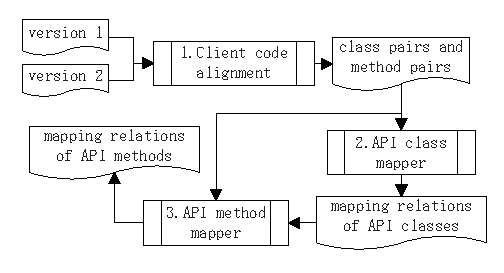
\includegraphics[scale=1,clip]{figure/approach.eps}\vspace*{-3ex}
 \caption{Overview of our approach}\vspace*{-3.5ex}
 \label{fig:approach}
\end{figure}
\subsection{Aligning Client Code}
\label{sec:approach:acc}

Given two versions of a project, the first step of our approach is
to align classes and methods of the two versions. Two aligned
classes or methods implement a similar functionality. As they
implement a similar functionality, APIs used by them may be
replaceable. For two versions of a project, our approach use name
similarities of two entities to align classes and methods of the two
versions. Here, we treat entity names (class/method names) defined
by the two versions of the project and entity names of third-party
libraries used by the two versions of the project differently. The
former often comes from the same programmer or the same team, or
programmers may refer to existing versions for naming entities such
as classes, methods, and variables. As a result, for the former,
using name similarity is often reliable to distinguish their
functionalities. For two entities, our approach chooses
Simmetrics\footnote{\url{http://sourceforge.net/projects/simmetrics/}}
to calculate similarities between their names.


Algorithm~\ref{alg:alignclasses} shows how our approach aligns
client code classes. The first step of the algorithm is to find
candidate class pairs by names. For two sets of classes ($C$ and
$C'$), the algorithm returns candidate pairs of classes ($M$) with
the maximum similarity and the similarity must be greater than a
predefined threshold. Some project may have many classes with the
same name, so $M$ may contain more than one pair for a class in a
version. To align those classes, the algorithm uses package names of
these classes to refine $M$ and returns only one pair with the
maximum similarity\footnote{For C\#, we refer to namespace names for
package names.}.

In each aligned class pair, our approach further aligns methods
within the class pair. The algorithm for methods is similar as the
algorithm for classes but relies on other criteria such parameter
numbers and names to refine candidate method pairs. These candidates
may contain more than one method pair due to overloading.

For the example shown in Section~\ref{sec:example}, our approach
correctly aligns the class named \CodeIn{IndexFiles} and the method
named \CodeIn{main} in Java to the class named \CodeIn{IndexFiles}
and the method named as \CodeIn{Main} in that their names are quite
similar.
\subsection{Mapping API classes}
\label{sec:approach:mappingtypes} The second step of our approach is
to mine mapping relations of API classes. As defined in
Section~\ref{sec:mapping}, mapping relations of API classes are used
to translate variables. Consequently, our approach mines mapping
relations of API classes based on how aligned client code declares
variables (\emph{i.e.}, fields of aligned classes, local variables
of aligned methods, and parameters of aligned methods). In
particular, for each aligned class pair $\Pair{c_1} {c_2}$, our
approach analyzes each field pair $\Pair{f_1}{f_2}$) and considers
$\Pair{f_1.type} {f_2.type}$ as one mined mapping relation of API
classes when the similarity between $f_1.name$ and $f_2.name$ is
greater than a threshold. Similarly, for each aligned method pair
$\Pair{m_1} {m_2}$, our approach analyzes each local variable pair
$\Pair{var_1}{var_2}$ and considers $\langle var_1.type,$ $
var_2.type\rangle$ as one mined mapping relation of API classes when
the similarity between $var_1.name$ and $var_2.name$ is greater than
a threshold. Also, our approach analyzes each parameter pair
$\langle para_1, $ $para_2\rangle$ of $m_1$ and $m_2$, and our
approach considers $\langle para_1.type,$ $para_2.type\rangle$ as
one mined mapping relation of API classes when the similarity
between $para_1.name$ and $para_2.name$ is greater than a threshold.
Here, the thresholds are the same as Section~\ref{sec:approach:acc}
in that they are all for names of client code.

For the example shown in Section~\ref{sec:example}, our approach
mines the mapping relation between \CodeIn{java.io.File} and
\CodeIn{System.IO.File- Info} based on the matched fields of Line 4
and Line 9. The mapping relation of API classes helps translate the
variable declared in Line 1 to the variable declared in Line 16.


\begin{algorithm}[t]
\begin{SmallOut}

\dontprintsemicolon
  \KwData{$C$ is the classes of a language; $C'$ is the classes
  of another language}
  \KwResult{$P$ is aligned pairs of classes}
  \Begin{
     $M \leftarrow findCandidateClassPairs(C, C')$\;
     \While{$M.size > 0 $}{
        \If{$M.size > 1$}{
            $M \leftarrow refineByPackageNames(M)$\;
         }
         \If{$M.size == 1$}{
                $P.add(M)$\;
                $C.remove(M[0].c)$\;
                $C'.remove(M[0].c')$\;
         }
         $M \leftarrow findCandidateClassPairs(C, C')$\;
     }
 }
 \end{SmallOut}

\label{alg:alignclasses} \caption{Align Classes Algorithm}
\end{algorithm}%\vspace*{-6ex}
%\begin{figure}[t]
%\centering
%\includegraphics[scale=0.4,clip]{figure/algorithm1.eps}\vspace*{-3ex}
% \label{alg:1}
%\end{figure}
\subsection{Mapping API methods}
\label{sec:approach:mappingtypes} The final step of our approach is
to mine mapping relations of API methods. This step has two major
sub-steps. First, our approach builds a graph for each client code
method. Second, our approach compares the two graphs of each paired
client code methods for mapping relations of API methods.

\begin{figure*}[t]
\centering
\includegraphics[scale=1.1,clip]{figure/graph.eps}\vspace*{-3ex}
 \caption
{\label{fig:graph}Built ATGs and the main steps of comparing
ATGs}\vspace*{-3.5ex}
\end{figure*}

\subsubsection{API transformation graph} An API transformation graph
(ATG) of a client code method ($m$) is a directed graph
($G\Triple{N_{data}}{N_{m}}{E}$). $N_{data}$ is a set of the fields
of $m$'s declaring class ($F$), the local variable of $m$ ($V$),
parameters of $m$ ($P_1$), parameters of methods called by
$m$($P_2$), and return values of all methods ($R$). $N_{m}$ is a set
of methods called by $m$. $E$ is a set of directed edges. An edge
($d_1\rightarrow d_2$) from a datum ($d_1 \in N_{data}$) to a datum
($d_2 \in N_{data}$) denotes the data dependency from $d_1$ to
$d_2$. An edge ($d_1 \rightarrow m_1$) from a datum ($d_1 \in
N_{data}$)  to a method ($ m_1 \in N_{m}$) denotes $d_1$ is a
parameter or a receiver of $m_1$. An edge ($m_1 \rightarrow d_1$)
from a method ($ m_1 \in N_{m}$) to a datum ($d_1 \in N_{data}$)
denotes $d_1$ is the return value of $m_1$.

We propose ATG for two considerations. One is for mining mapping
relations of method inputs correctly. The inputs of two API methods
that satisfy all criteria of mapping relations may have different
orders and positions. For example, \CodeIn{java.math.BigDecimal.
multiply(BigDecimal)} has a receiver ($v_1$) and a parameter
($p_1$); \CodeIn{System.Decimal.Multiply(Decimal, Decimal)} has two
parameters ($p_2$ and $p_3$). Here, $v_1$ is mapped with $p_2$, and
$p_1$ is mapped with $p_3$. As ATG describes inputs of API methods,
our approach is able to deal with the problem of mapping inputs. The
other is for mining mapping relations of merging API methods. As ATG
describes data dependencies among inputs and outputs, our approach
is able to mine mapping relations for merged API methods as shown in
Figure~\ref{fig:example}.

\subsubsection{Building API transformation graphs} The first sub-step
builds an ATG for each method. The graph contains details such as
inputs and outputs for each client code method. In particular, for
each method, our approach first builds subgraph for its variables,
API methods, and field accesses according to the rules as follows:

%First, programming languages typically provide a huge set of APIs,
%and it is difficult to build mapping relations for all APIs
%manually. Second, some API methods have multiple parameters, and
%some parameters cannot be mapped directly one by one in orders. For
%example, \CodeIn{org.w3c.dom.Element.getAttributeNS()} and
%\CodeIn{System.Xml.XmlElement.GetAttribute()} both have two
%parameters, but the two parameters are inverse by their meanings.
%Third, one API method in one language may be mapped to more than one
%API method in other languages. For example, \CodeIn{java.util.
%LinkedList.removeLast()} returns the last value, and \CodeIn{System.
%Collections.Generic.LinkedList.RemoveLast()} does not return any
%values. To get that value, C\# programmers need to call more APIs,
%and thus one API method of Java is mapped to serval API methods of
%C\#.



%
%One challenge to mine mapping relations of two API methods lies in
%how to map their inputs correctly. Here, our approach both the
%receiver and the parameters of a method as the inputs of a
%method. Inputs of two API methods may be matched but are not in the
%same order. For example, as shown in Section~\ref{sec:example},
%\CodeIn{java.io. File.exist()} has a receiver whereas
%\CodeIn{System.IO.File.Exist()} has no receiver but a
%parameter. In addition, parameter orders may be quite different. For
%example, the parameter order of \CodeIn{org.w3c.
%dom.Element.getAttributeNS()} is inverse with the parameter order of
%\CodeIn{System.Xml.XmlElement.GetAttribute()}. To deal with the
%preceding problem,



(1) $f\in F\cup V \cup P_1 \Rightarrow $
%\restylefloat{figure}
%\begin{figure}[H]\vspace*{-5ex}
%\begin{center}
\includegraphics[scale=0.7,clip]{figure/rule1.eps}%\vspace*{-1.5ex}
%\end{center}

Our approach adds used variables of a client code method as these
variables are useful to analyze data dependencies among API methods.

(2) $T_0\ m (T_1 p_1, \ldots, T_n p_n) \Rightarrow $
%\begin{figure}[h]

\begin{center}
\includegraphics[scale=0.7,clip]{figure/rule2.eps}%\vspace*{-1.5ex}
\end{center}

%\end{figure}

Our approach adds API methods called by a client code method to the
built graph. For each API method $m$, $T$ is the declaring class of
$m$. Our approach does not add a receiver nodes for static methods,
and our approach does not add parameter nodes for methods without
parameters.

(3) $f.x, f\in F\cup V\Rightarrow $
%\begin{figure}[h]

\begin{center}
\includegraphics[scale=0.7,clip]{figure/rule3.eps}%\vspace*{-1.5ex}
\end{center}

As Java often uses getters and setters whereas C\# often use field
accesses, our approach treats field accesses as a special type of
method calls. In the preceding sub-graph, $f$ is a variable whose
type is $T_1$, and $T_0$ is the type of $f.x$.


Our approach further connects the built subgraphs through data
dependencies among built sub-graphs. In particular, our approach
analyzes source files of a client code method statement by statement
and adds edges according to the rules as follows:

(4) $x=y, x\in F\cup V\wedge y\in F\cup V \Rightarrow $

\begin{center}
\includegraphics[scale=0.7,clip]{figure/rule4.eps}%\vspace*{-1.5ex}
\end{center}

Our approach adds an edge from $y$ to $x$ if $y$ is assigned to $x$.
The edge denotes the data dependency from $y$ to $x$.

(5) $x=m(), x\in F\cup V \Rightarrow $

%\begin{figure}[h]\vspace*{-1.5ex}
\begin{center}
\includegraphics[scale=0.7,clip]{figure/rule5.eps}%\vspace*{-1.5ex}
\end{center}

Our approach adds an edge from $m$ to $x$ if $m$'s return value is
assigned to $x$. The edge denotes the data dependency from $m$'s
return value to $x$.


(6) $m(x)\Rightarrow$

%\begin{figure}[h]\vspace*{-1.5ex}
\begin{center}
\includegraphics[scale=0.7,clip]{figure/rule6.eps}%\vspace*{-1.5ex}
\end{center}

Our approach adds an edge from $x$ to $m$'s parameter node if $x$ is
a parameter of $m$. The edge denotes the data dependency from $x$ to
$m$'s parameter.

(7) $m_2(m_1(x))\Rightarrow$

%\begin{figure}[h]\vspace*{-1.5ex}
\begin{center}
\includegraphics[scale=0.7,clip]{figure/rule7.eps}%\vspace*{-1.5ex}
\end{center}

Our approach adds an edge from $m_1$'s return value node to $m_2$'s
parameter node if $m_1$ is used as a parameter of $m_2$. The edge
denotes the data dependency from $m_1$'s return value node to
$m_1$'s parameter.


(8) $x.m()\Rightarrow$
\begin{center}
\includegraphics[scale=0.7,clip]{figure/rule8.eps}%\vspace*{-1.5ex}
\end{center}

Our approach adds an edge from $x$ to $m$ if $x$ is an variable that
is related to $m$. The edge denotes the data dependency from $x$ to
$m$'s parameter.

(9) $x=y\ binop\ z\ binop\ \ldots, binop\in \{+,-,*,/\} \Rightarrow
$


\begin{center}
\includegraphics[scale=0.7,clip]{figure/rule9.eps}%\vspace*{-1.5ex}
\end{center}

Our approach adds edges from $y$, $z$, and others to $x$ if these
variables are connected by bin operations and the return value is
assigned to $x$. The edge denotes the data dependency from $y$, $z$,
and other variables to $x$. For simplicity, our approach ignores
\emph{binop} info. We further discuss the issue in
Section~\ref{sec:discuss}.

For each client code method, our approach applies the preceding
rules by statement orders. For each statement, our approach applies
the rules by depths of built abstract syntax tree from the lower to
the higher. For the two source files shown in
Section~\ref{sec:example}, Figure~\ref{fig:graph} (a) shows the
partial ATG of \CodeIn{IndexFiles.cs}, and Figure~\ref{fig:graph}
(b) shows the partial ATG of \CodeIn{IndexFiles.java}.
Figure~\ref{fig:graph} also lists corresponding line numbers of each
sub-graph. In particular, for Line 4 and Line 9, our approach
applies Rule 2 and Rule 6 to build corresponding sub-graphs. For
Line 6 and Line 7, our approach applies Rule 2 and Rule 8 to build
corresponding sub-graphs. For Line 12 and Line 15, our approach
applies Rule 2, Rule 3, and Rule 6 to build corresponding
sub-graphs.
\begin{algorithm}[t]
\begin{SmallOut}
\label{alg:mapATG} \dontprintsemicolon
  \KwData{$G$ is the ATG of a method ($m$); $G'$ is the ATG of $m$'s mapped method.}
  \KwResult{$S$ is a set of mapping relations for API methods}
  \Begin{
     $P \leftarrow findVarPairs(m, m')$\;
     \For{Pair p in P}{
        $SM \leftarrow G.nextMethods(p.sharp)$\;
        $JM \leftarrow G.nextMethods(p.java)$\;
        $\Delta S = mapping(SM, JM)$\;
        \While{$\Delta S \neq \phi| \Delta SM \neq \phi| \Delta JM \neq \phi$}{
            $S.addAll(\Delta S)$\;
             \For{Method sm in SM}{
                 \If{$sm.isMapped$}{
                    $SM.replace(sm, sm.nextMethod())$\;
                  }\Else{
                    $SM.replace(sm, sm.mergeNextMethod())$\;
                  }
             }
             \For{Method jm in JM}{
                 \If{$jm.isMapped$}{
                    $JM.replace(jm, jm.nextMethod())$\;
                  }\Else{
                    $JM.replace(jm, Jm.mergeNextMethod())$\;
                  }
             }
             $\Delta S = mapping(SM, JM)$\;
        }
     }
 }
 \end{SmallOut}
\caption{ATG Comparison Algorithm}
\end{algorithm}

\subsubsection{Comparing API transformation graphs} The
second sub-step compares each pair of built ATGs for mapping
relations of API methods. As shown in Figure~\ref{fig:example}, two
mapped API methods have (1) the same functionality, (2) the mapping
relations of inputs, and (3) the mapping relations of returns. As
two mapped API methods satisfy the preceding three criteria, they
are replaceable in client code and thus are useful to aid language
migration.

Algorithm~\ref{alg:mapATG} shows the main steps of comparing ATGs
for mining mapping relations of API methods. For each method pair
$\langle m, m'\rangle$, our algorithm first finds matched variable
pairs and matched constant pairs of $F$, $V$, and $P_1$ of $m$ and
$m'$. For two variables, our algorithm considers them matched when
the similarity between two variables is greater than a threshold.
For constants, our algorithm considers them matched when the two
constants have exactly the same value. For each variable pair and
each constant pair, our algorithm finds the first two methods ($jm$
and $sm$) that use the two variables or the two constants as inputs.
Our algorithm considers $jm$ and $sm$ mapped when they satisfy the
following criteria:

\emph{inputs}: (1) the total number of $jm$'s receiver and
parameters equal the total number of $sm$'s receiver and parameters;
(2) each receiver and each parameter are mapped. Here, our algorithm
considers two inputs matched if the two inputs come from two matched
variables/constants or two outputs of two matched API methods.

\emph{functionalities}: The similarity between the name of $jm$ and
the name of $sm$ is greater than a threshold.

\emph{outputs:} The output of $jm$ and the output of $sm$ are mapped
API classes.

If a method is mapped, our approach replaces the method with its
next connected method. If a method is not mapped, our approach
merges the next connected method to this method. As our approach
merges some methods, both $jm$ and $sm$ may be two merged API
methods. For two merged API methods, and our algorithm uses the
maximum similarity of method names between $jm$ and $sm$ as the
similarity of their functionalities. Our algorithm continues until
$S$, $SM$, and $JM$ do not change anymore.


For example, the numbers within circles of Figure~\ref{fig:graph}
show the main steps to mine the mapping relations of API methods as
shown in Figure~\ref{fig:example}. The main steps are as follows:

\emph{S1: mapping parameters, fields, local variables, and
constants.} For the two graphs of each method pair, this step maps
variables such as parameters, fields, and local variables by names
and maps constants by values. For the preceding example, this step
maps two constants as shown by the first red arrow of
Figure~\ref{fig:graph} since the two constants have the same values
as \CodeIn{index}.

\emph{S2: mapping inputs of API methods.} For each variable pair,
this step traces to the first connected two API methods and tries to
map all the parameters and the receivers of the two API method. For
the preceding example, this step maps the parameter named as
\CodeIn{filename} to the parameter named as \CodeIn{arg0} as they
are of the same type and they connect to the mapped constants.

\emph{S3: mapping outputs of API methods.} After inputs are mapped,
this step further maps outputs of API methods. If it fails to map
outputs, this step further merges the next API method and tries to
map output of merged API methods. For the preceding example, as the
output of \CodeIn{System.IO.FileInfo()} is not mapped to the output
of \CodeIn{java.io.File.File()}, this step further merges the next
API methods until it finds a match. The arrows marked as ``3"" of
Figure~\ref{fig:graph} shows the matched outputs. These outputs are
of matched API classes.

\emph{S4: mapping functionalities.} After inputs and outputs are
both mapped, this step further maps functionalities of those merged
methods. Give two merged methods with mapped inputs and outputs,
this step use the maximum similarity of method names as the measure
for their functionalities. In the preceding example, this step maps
the two merged methods shown in Figure~\ref{fig:graph} (a) to the
merged methods of the \CodeIn{java.io.File.exist()} as the three
merged methods all contain a method named as ``exist''.

After comparing the graph shown in Figure~\ref{fig:graph} (a) with
the graph shown in Figure~\ref{fig:graph} (b), our approach mines
the mapping relation as shown in Figure~\ref{fig:example} by merging
variables between API methods.
